\chapter{Versuchsauswertung}\label{s:auswertung}

\section{Reine Ausblasung (AK)}
\label{s:reineAusblasung}

In \abschn{s:reineAusblasung} wurde das Profilmodell mit den glatten Welle im Windkanal eingebaut.Es gab keine Rotation bei den Wellen und der Versuch wurde mit den glatten Wellen ohne Aktuation durchgef\"uhrt. Der Volumenstrom wurde so eingestellt, dass
die folgenden $C_{\mu}$  Werte erreicht werden. Es wurde $C_{w}$ mit diesen vier verschiedenen $C_{\mu}$ Werte gemessen.Die Ergbnisse sind wie folgt:
\begin{table}[h]
	\centering
	\begin{tabular}{lr}
		\toprule
		$C_{\mu}$ & $C_{w}$ \\
		\midrule
		0.00 & 0.876\\
		0.16 & 0.606\\
		0.32 & 0.477\\
		0.48 & 0.399\\
		0.69 & 0.331\\
		\bottomrule
	\end{tabular}
	\caption{$C_{w}$ und $C_{\mu}$ mit der glatten Welle ohne Aktuation }
	\label{tab:Cw-Cmu_Kon1}
\end{table}


Die \abb{fig:Cw-Cmu_Konf1} zeigt die Funktion von Widerstandsbeiwert \"uber Impulsbeiwert f\"ur die glatte welle ohne Atuation:
\begin{figure}[h]
	\centering
	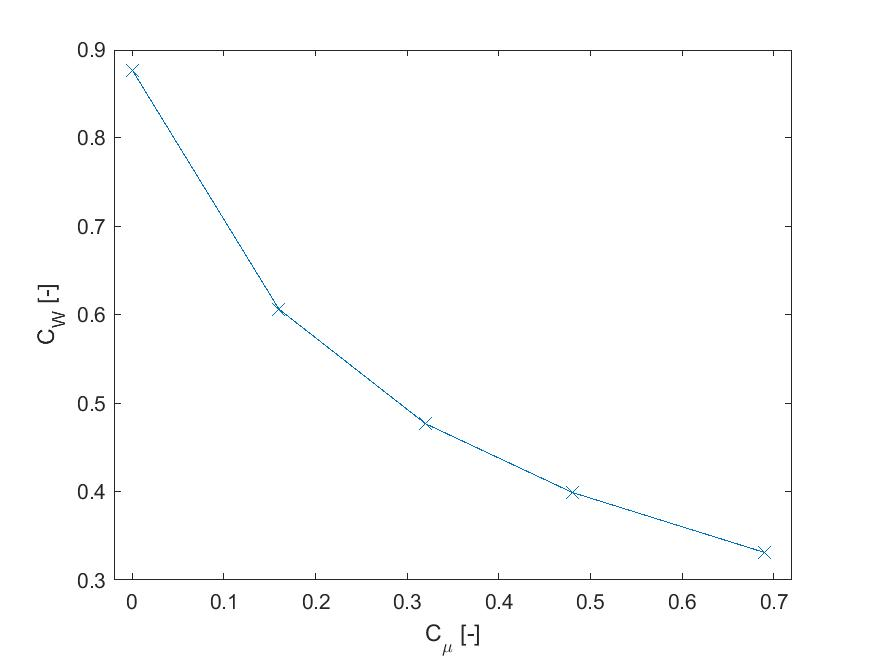
\includegraphics[width=0.5\textwidth]{Cw_ueber_Cmu_ohne_n.jpg}
	\caption{$C_{w}$  \"uber $C_{\mu}$ mit den glatten Wellen ohne Aktuation }
	\label{fig:Cw-Cmu_Konf1}
\end{figure}

Wie man im Diagramm betrachtet, ist es ein deutlicher Abfall von $C_{w}$ mit steigendem $C_{\mu}$.
F\"ur den Versuch mit den ovalen Wellen wurde $C_{\mu}$ Werte f\"ur die Verschiedenen Luftdr\"ucke berechnet. Unten sind die Auswertungen f\"ur $C_{w}$:
 
\begin{table}[h]
	\centering
	\begin{tabular}{lrr}
		\toprule
		Luftdruck [kPa] & $C_{\mu}$ & $C_{w}$ \\
		\midrule
		0 & 0.00 & 0.805\\
		1 & 0.06 & 0.610\\
		2 & 0.27 & 0.594\\
		3 & 0.42 & 0.577\\
		4 & 0.58 & 0.455\\
		\bottomrule
	\end{tabular}\\
	\caption{Luftdruck, $C_{w}$  und $C_{\mu}$ f\"ur die glatten und ovalen Wellen ohne Aktuation}
	\label{tab:Cw-Cmu_Konf1+2}
\end{table}


Die \abb{fig:Cw-Cmu_Konf1+2} zeigt den Verlauf $C_{w}$ \"uber $C_{\mu}$ f\"ur die beiden Konfigurationen:
\begin{figure}[h]
	\centering
	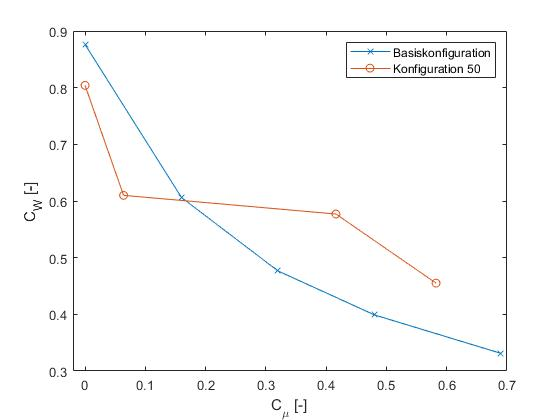
\includegraphics[width=0.5\textwidth]{Cw_ueber_Cmu_ohne_n_beideKonf.jpg}
	\caption{$C_{w}$  \"uber $C_{\mu}$ mit den glatten Wellen ohne Aktuation }
	\label{fig:Cw-Cmu_Konf1+2}
\end{figure}

Wie man im Diagramm sieht, f\"allt auch $C_{w}$  mit steigendem $C_{\mu}$  mit den ovalen Wellen ab.
\\
Im Vergleich mit den glatten Wellen sind die Widerstandsbeiwerte bei Impulskoeffizient im Bereich von 0 bis 0.16  in den ovalen Wellen niedriger als den glatten Wellen. Aber ab dem Punkt $C_{\mu}$= 0.16 sinkt der Widerstandsbeiwert der glatten Wellen st\"arker ab. Aus diesem Grund sind die glatten Wellen ohne Aktuation bei den gr\"o\ss{}eren Impulskoeffiziente zu empfehlen.
    




\label{sec:ErgebnisseKonstanteAktuation}

\section{Periodische Aktuation}


%\subsection{Ausrichtungsmessungen (FT)}
%\label{subs:Vorueberlegungen}
%
%Um die periodische Aktuation zu erm"oglichen, werden die glatten, zylindrischen Wellen aus Aluminium gegen die in \abschn{s:rotierendeWalzen} beschriebenen Wellen getauscht.
%
%Nach dem Einbau wurde erneut die Druckverteilung auf der Oberfl"ache des Modells vorgenommen, um eine optimale Postion des Modells ohne Anstellwinkel zu gew"ahrleisten. Die Ergebnisse sind in \abb{fig:Oberflaechendruckverteilung 50}
%zu sehen.
%
%	\begin{figure}[h]
%	\centering
%	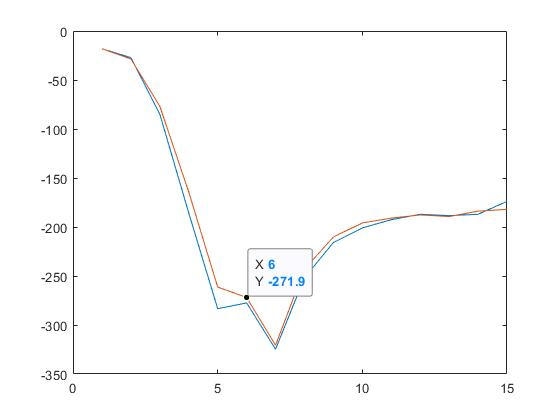
\includegraphics[width=0.8\textwidth]{Oberflaechendruckverteilung50.jpg}
%	\caption{Oberfl"achendr"ucke beim eingebauten Modell mit Teflonwalzen}
%	\label{fig:Oberflaechendruckverteilung 50}
%	\end{figure}
%
%Die D"rucke an der Ober- und Unterseite sind hier wieder gespiegelt und "ubereinandergelegt dargestellt. Der erste Messpunkt entspricht dabei der Druckmessbohrung, die mittig an der Vorderseite eingebracht ist.
%
%Die gr"o\ss{}te Abweichung erf"ahrt der Druck an Ober- und Unterseite genau dort, wo auf beiden Seiten das Zackenband angebracht wurde. Der lokale, jeweilige Abstand der Druckmessbohrung zum Zackenband ist allerdings oben und unten nicht komplett einheitlich. Dies hat zur Folge, dass das Str"omungsverhalten an diesen Orten voneinander abweicht, wodurch die Differenz zu erkl"aren ist.
%Da die Druckmessbohrungen im Folgenden keine gro\ss{}e Relevanz haben, ist diese Ungleichm"a\ss{}igkeit kein Problem.
%
%Weiterhin ergibt sich allerdings im Unterschied zu den Messungen der Oberfl"achendr"ucke in \abschn{sec:ErgebnisseKonstanteAktuation} eine leichte Druckerh"ohung an der Oberseite zur letzten Druckmessbohrung hin.
%Auch in der Arbeit von \emph{Bilges} \,\cite{Bilges.2018}, die das gleiche Modell als Gegenstand der Untersuchung hatte,ist eine "ahnliche Entwicklung bei niedrigeren Reynoldszahlen als 50.000 zu sehen gewesen.
%Die beschriebene Tendenz war aber bei h"oheren Reynoldszahlen wieder kaum wahrnehmbar.
%
%
%Diese Erscheinung lie\ss{} sich auch nach "Uberpr"ufung der Schl"auche und Bohrungen auf Verunreinigungen bzw. Verstopfungen und mehreren Nachjustierungen der Modellpostion nicht beseitigen.
%
%Auch der m"ogliche Einfluss der oberen und unteren Walze auf diese Werte durch etwaiges leichtes Aufbiegen der Spalte in variierenden Walzenstellungen wurde ohne positive Ver"anderung getestet.
%
%Das Auseinanderstreben der Messwerte ist somit wahrscheinlich auf die in \cite{Bilges.2018} angef"uhrten einseitigen Fertigungstoleranzen und Unebenheiten zur"uckzuf"uhren, welche je nach individueller Einstellung der Spalte bei den verschiedenen Walzenpaaren unterschiedlich stark zum Vorschein kommen.
%
%Da an den anderen Messpunkten Ober- und Unterseite sehr "ahnliche Werte liefern, kann davon ausgegangen werden, dass das Modell symmetrisch in der Anstr"omung platziert ist.
%
%
%Die eigentlichen Messreihen gestalteten sich bei dieser Konfiguration aus verschiedenen Gr"unden als schwieriger und aufw"andiger als bei der Konfiguration aus \abschn{sec:ErgebnisseKonstanteAktuation}.
%
%%Damit lokale
%%
%%Phasenungleicheit bei der Wellenrotation.:
%%
%%Da nicht ausgeschlossen werden kann, dass die beiden Walzen beim Hochfahren der Drehzahl asynchron laufen und sich eine phasenversetzte Aktuation an Ober- und Unterseite ergibt, wurden zu jeder Kombination der Messparameter mehrere Messungen durchgef"uhrt.
%%
%%Eine 
\section{Effizienzbetrachtung}
